\subsection{Study selection}
Screening identified controlled trials of MDMA, LSD, psilocybin, and ayahuasca that reported harmonized AE outcomes. Reasons for exclusion most commonly included uncontrolled designs, duplicate publications, and inadequate AE capture. The final analytic dataset comprised 487 session-level contrasts (149 LSD, 160 MDMA, 162 psilocybin, and 16 ayahuasca) and 166 follow-up contrasts (108 LSD and 58 MDMA) derived after applying the prespecified reference-arm policy in \Cref{tab:study-characteristics}.

\subsection{Study characteristics}
Included trials spanned one to six distinct dose tiers per molecule and covered both acute (session) and delayed (follow-up) assessments. Session-level analyses were available for all four molecules, whereas follow-up contrasts were confined to LSD and MDMA. Arm-level contributions, including the number of unique dose conditions per time window, are summarised in \Cref{tab:study-characteristics}.

\subsection{Primary synthesis of adverse events}
Random-effects pooling across molecules showed consistent elevation of AE risk relative to the designated reference arms, as illustrated by the combined forest plot in \Cref{fig:overall-forest}. Molecule-specific heterogeneity estimates appear in \Cref{tab:meta-summary}, where session-level $I^2$ ranged from 17.9\% (MDMA) to 52.6\% (psilocybin). Follow-up estimates for LSD (108 contrasts) retained statistical significance with null heterogeneity, whereas MDMA follow-up models (58 contrasts) trended toward significance but did not cross the conventional threshold ($p=0.057$). Corresponding significance counts are provided in \Cref{tab:topline-summary}.

\IfFileExists{figures/forest_combined_all_molecules.pdf}{%
  \begin{figure}[ht]
    \centering
    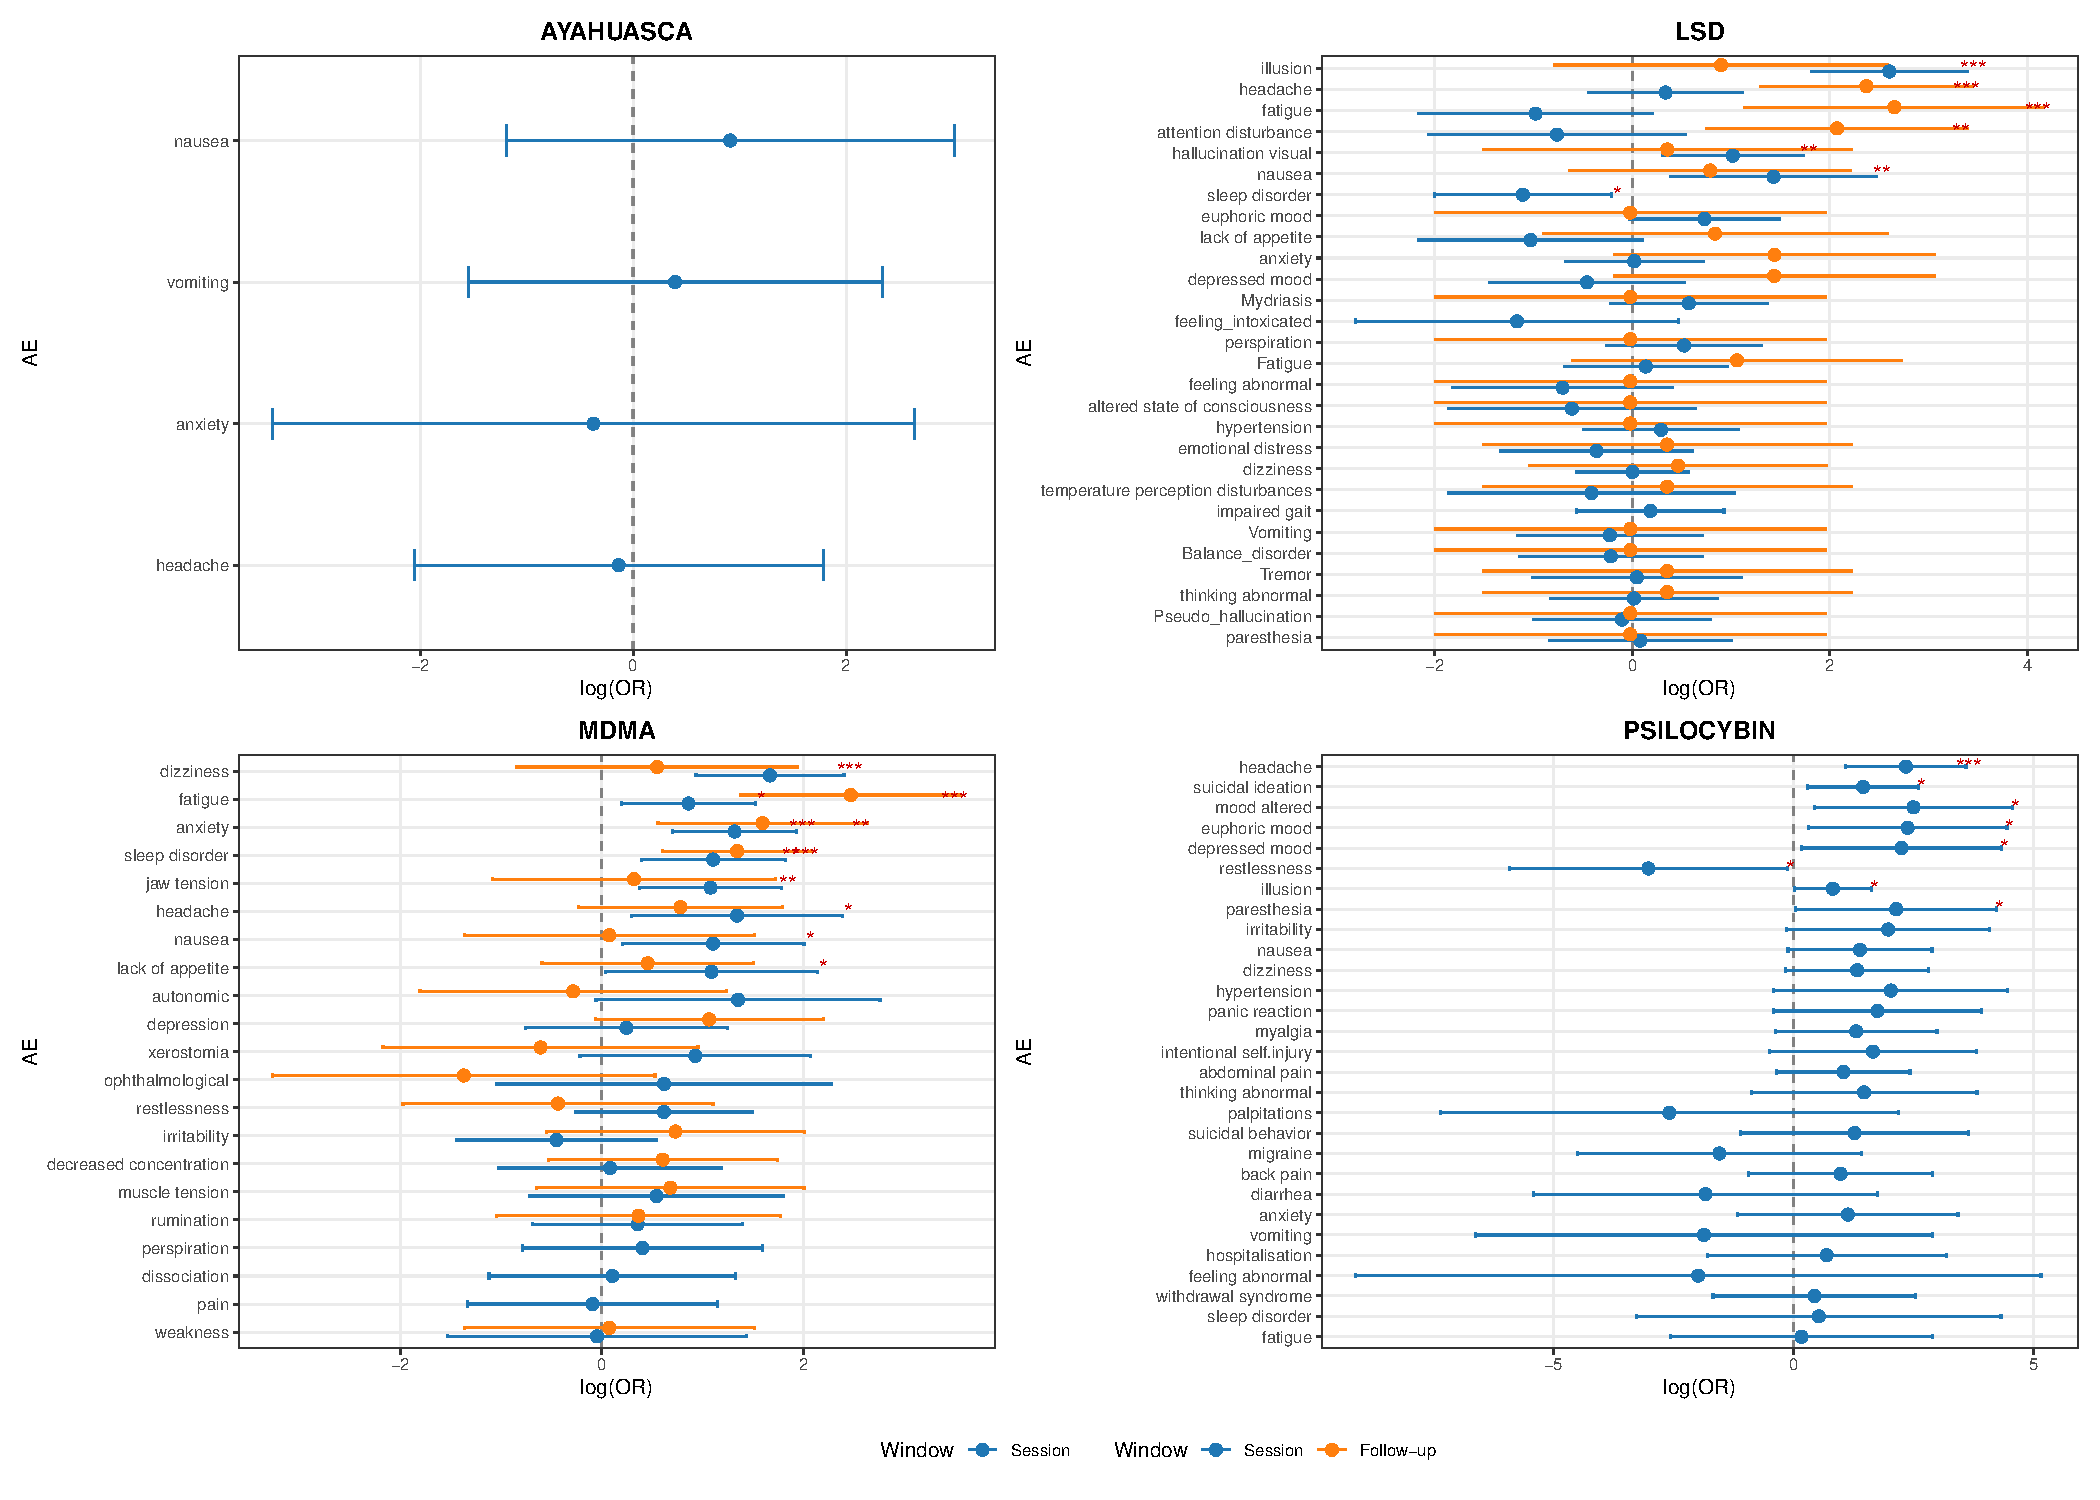
\includegraphics[width=\linewidth]{figures/forest_combined_all_molecules.pdf}
    \caption{Random-effects forest plot summarising pooled AE risk ratios across molecules and time windows.}
    \label{fig:overall-forest}
  \end{figure}
}{}

\IfFileExists{tables/compare_by_molecule_overall.tex}{%
  \begin{table}[ht]
    \centering
    \caption{Random-effects meta-analysis summaries by molecule and time window. $k$ denotes the number of contrasts contributing to each model.}
    \label{tab:meta-summary}
    \begin{tabular}{lrrrlrrrl}
\toprule
  Molecule &  k (session) &  I2 (session) &  tau2 (session) & p\_overall (session) &  k (follow) &  I2 (follow) &  tau2 (follow) & p\_overall (follow) \\
\midrule
       LSD &          149 &     19.839319 &        0.313555 &               <0.001 &       108.0 &          0.0 &       0.000000 &               0.002 \\
      MDMA &          197 &     17.988909 &        0.282440 &               <0.001 &        58.0 &          0.0 &       0.000001 &               0.057 \\
Psilocybin &          162 &     52.628558 &        1.707960 &               <0.001 &         NaN &          NaN &            NaN &                     \\
\bottomrule
\end{tabular}

  \end{table}
}{}

\IfFileExists{tables/compare_topline_molecule.tex}{%
  \begin{table}[ht]
    \centering
    \caption{Top-line significance outcomes and counts of significant adverse events by molecule and time window.}
    \label{tab:topline-summary}
    \begin{tabular}{lrllrrl}
\toprule
  Molecule &  \# Sig. AEs (session) & Session p-value & Session sig. &  \# Sig. AEs (follow) &  Follow-up p-value & Follow-up sig. \\
\midrule
       LSD &                      2 &          <0.001 &          *** &                   0.0 &              0.002 &             ** \\
      MDMA &                      1 &          <0.001 &          *** &                   0.0 &              0.057 &            NaN \\
Psilocybin &                      1 &          <0.001 &          *** &                   NaN &                NaN &            NaN \\
\bottomrule
\end{tabular}

  \end{table}
}{}

\IfFileExists{tables/compare_agg_by_molecule.tex}{%
  \begin{table}[ht]
    \centering
    \caption{Dose--response omnibus tests (QM) by molecule and time window.}
    \label{tab:dr-omnibus}
    \begin{tabular}{lrrlrrl}
\toprule
  Molecule &  k (session) &  QM (session) & p (session) &  k (follow) &  QM (follow) & p (follow) \\
\midrule
       LSD &          149 &     11.362791 &      <0.001 &       108.0 &     4.701383 &      0.002 \\
      MDMA &          197 &      5.157476 &      <0.001 &        58.0 &     0.666592 &      0.057 \\
Psilocybin &          162 &     19.134286 &      <0.001 &         NaN &          NaN &            \\
\bottomrule
\end{tabular}

  \end{table}
}{}

\subsection{Per-adverse-event findings}
Harmonized per-AE models indicated that only a subset of AE terms demonstrated clear dose-related elevations. Coverage of adverse-event terms across molecules is detailed in \Cref{tab:ae-coverage}, highlighting repeated assessments for anxiety, headache, nausea, fatigue, and related autonomic symptoms. Significant session-level findings predominantly involved autonomic and gastrointestinal symptoms for MDMA, nausea and headache for LSD, and fatigue and hypertension for psilocybin, with corresponding $p$-values documented in \Cref{tab:cmp_ae_molecule}. Overlay plots in \Cref{fig:per-ae-overlays} show the alignment of spline-based dose--response curves across molecules for shared AE terms.

\IfFileExists{tables/compare_agg_by_ae_molecule.tex}{%
  \begin{table}[p]
    \centering
    \footnotesize
    \caption{Number of contrasts contributing to each adverse-event model by molecule and time window.}
    \label{tab:ae-coverage}
    \begin{tabular}{llrr}
\toprule
                      Adverse event &   Molecule &  k (session) &  k (follow) \\
\midrule
                   Balance_disorder &        LSD &            4 &         4.0 \\
                            Fatigue &        LSD &            4 &         4.0 \\
                          Mydriasis &        LSD &            4 &         4.0 \\
               Pseudo_hallucination &        LSD &            4 &         4.0 \\
                             Tremor &        LSD &            4 &         4.0 \\
                           Vomiting &        LSD &            4 &         4.0 \\
                     abdominal pain & Psilocybin &            4 &         NaN \\
     altered state of consciousness &        LSD &            4 &         4.0 \\
                            anxiety &        LSD &            7 &         4.0 \\
                            anxiety &       MDMA &           13 &         4.0 \\
                            anxiety & Psilocybin &            7 &         NaN \\
              attention disturbance &        LSD &            5 &         6.0 \\
                          autonomic &       MDMA &            5 &         NaN \\
                          back pain & Psilocybin &            3 &         NaN \\
            decreased concentration &       MDMA &            4 &         3.0 \\
                     depressed mood &        LSD &            4 &         4.0 \\
                         depression &       MDMA &            6 &         3.0 \\
                           diarrhea & Psilocybin &            3 &         NaN \\
                       dissociation &       MDMA &            4 &         NaN \\
                          dizziness &        LSD &            6 &         5.0 \\
                          dizziness &       MDMA &            7 &         NaN \\
                          dizziness & Psilocybin &            4 &         NaN \\
                 emotional distress &        LSD &            5 &         4.0 \\
                      euphoric mood &        LSD &            4 &         4.0 \\
                            fatigue &       MDMA &           11 &         4.0 \\
                            fatigue & Psilocybin &            5 &         NaN \\
                   feeling abnormal &        LSD &            5 &         4.0 \\
               hallucination visual &        LSD &            4 &         4.0 \\
                           headache &        LSD &            8 &         6.0 \\
                           headache &       MDMA &           11 &         4.0 \\
                           headache & Psilocybin &            9 &         NaN \\
                       hypertension &        LSD &            4 &         4.0 \\
                       hypertension & Psilocybin &            4 &         NaN \\
                           illusion &        LSD &            4 &         4.0 \\
                      impaired gait &        LSD &            3 &         NaN \\
                       irritability &       MDMA &            5 &         3.0 \\
                        jaw tension &       MDMA &           10 &         NaN \\
                   lack of appetite &        LSD &            4 &         4.0 \\
                   lack of appetite &       MDMA &            8 &         4.0 \\
                           migraine & Psilocybin &            3 &         NaN \\
                     muscle tension &       MDMA &            7 &         3.0 \\
                            myalgia & Psilocybin &            3 &         NaN \\
                             nausea &        LSD &            5 &         5.0 \\
                             nausea &       MDMA &            9 &         NaN \\
                             nausea & Psilocybin &            8 &         NaN \\
                   ophthalmological &       MDMA &            4 &         NaN \\
                               pain &       MDMA &            6 &         NaN \\
                        paresthesia &        LSD &            4 &         4.0 \\
                       perspiration &        LSD &            5 &         4.0 \\
                       perspiration &       MDMA &            6 &         NaN \\
                       restlessness &       MDMA &            8 &         NaN \\
                         rumination &       MDMA &            5 &         NaN \\
                     sleep disorder &       MDMA &           12 &         8.0 \\
                     sleep disorder & Psilocybin &            4 &         NaN \\
                  suicidal ideation & Psilocybin &            6 &         NaN \\
temperature perception disturbances &        LSD &            5 &         4.0 \\
                  thinking abnormal &        LSD &            5 &         4.0 \\
                           weakness &       MDMA &            3 &         NaN \\
                         xerostomia &       MDMA &            4 &         NaN \\
\bottomrule
\end{tabular}

  \end{table}
}{}

\IfFileExists{figures/master_dr_by_ae-session.pdf}{%
  \begin{figure}[ht]
    \centering
    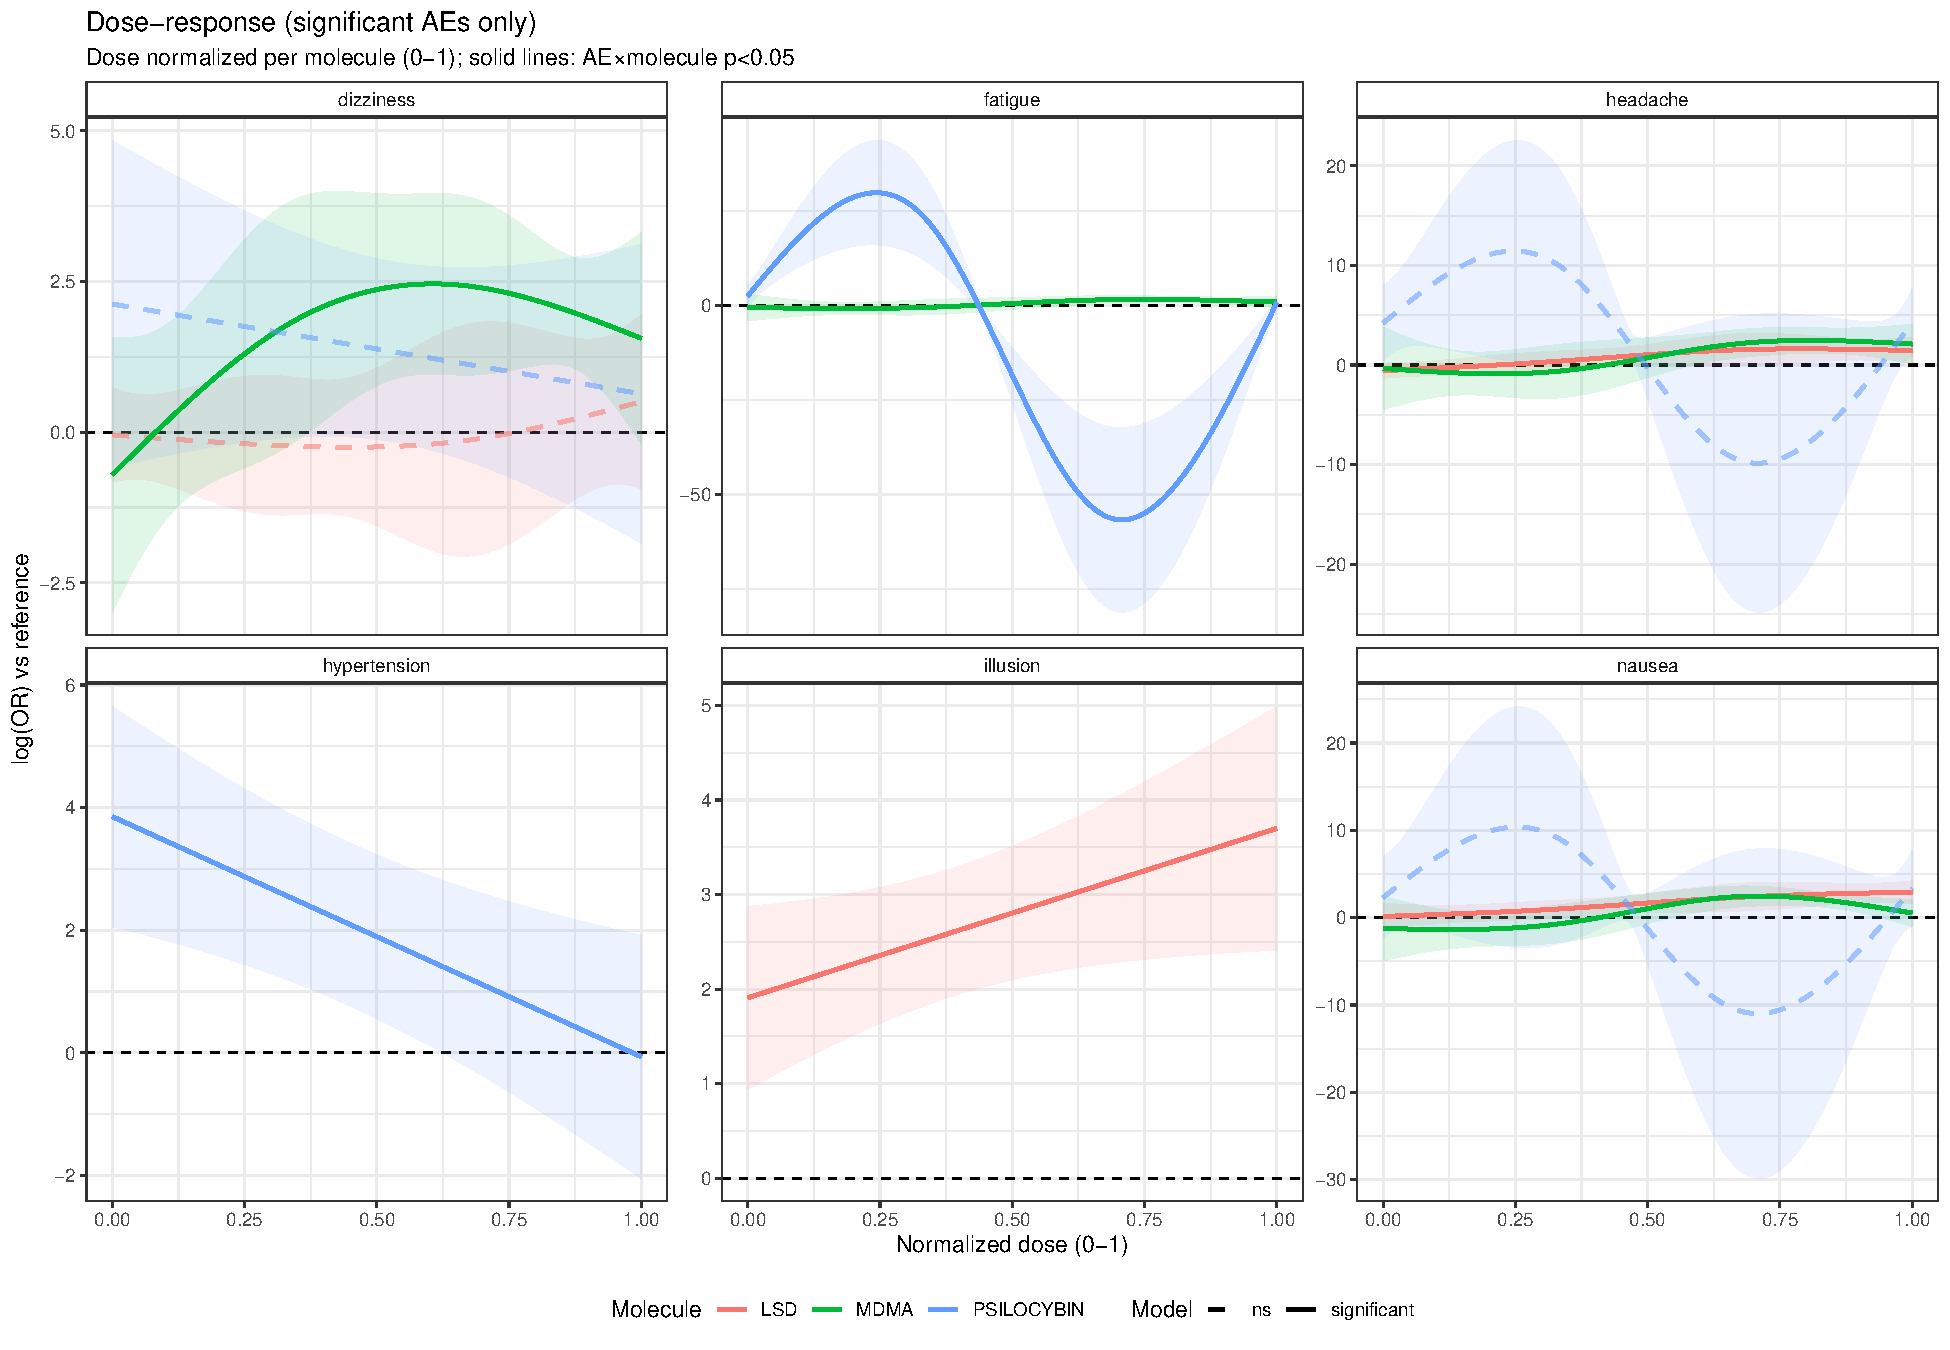
\includegraphics[width=\linewidth]{figures/master_dr_by_ae-session.pdf}
    \caption{Session-level dose--response overlays for harmonized AE terms observed across multiple molecules.}
    \label{fig:per-ae-overlays}
  \end{figure}
}{}

\IfFileExists{../results_compare/tables/compare_by_ae_molecule.tex}{%
  \begin{table}[p]
    \centering
    \footnotesize
    \caption{Per-adverse-event meta-analytic summaries by molecule and time window.}
    \label{tab:cmp_ae_molecule}
    \begin{table}[ht]
\centering
\caption{Per-AE comparison by molecule: session vs follow-up p-values.}
\label{tab:cmp_ae_molecule}
\begin{tabular}{llll}
\toprule
molecule & ae_term & session & follow \\
\midrule
LSD & anxiety & p=0.713  &  \\
LSD & attention disturbance & p=0.526  & p=0.15  \\
LSD & dizziness & p=0.89  & p=0.912  \\
LSD & emotional distress & p=0.256  &  \\
LSD & feeling abnormal & p=0.372  &  \\
LSD & headache & p=0.0104 * & p=0.629  \\
LSD & nausea & p=0.025 * & p=0.885  \\
LSD & perspiration & p=0.511  &  \\
LSD & temperature perception disturbances & p=0.774  &  \\
LSD & thinking abnormal & p=0.662  &  \\
MDMA & anxiety & p=0.0724  &  \\
MDMA & autonomic & p=0.0719  &  \\
MDMA & depression & p=0.0456 * &  \\
MDMA & dissociation & p=0.362  &  \\
MDMA & dizziness & p=0.147  &  \\
MDMA & fatigue & p=0.159  &  \\
MDMA & headache & p=0.00654 ** &  \\
MDMA & irritability & p=0.284  &  \\
MDMA & jaw tension & p=0.491  &  \\
MDMA & lack of appetite & p=0.156  &  \\
MDMA & muscle tension & p=0.509  &  \\
MDMA & nausea & p=0.336  &  \\
MDMA & ophthalmological & p=0.196  &  \\
MDMA & pain & p=0.129  &  \\
MDMA & perspiration & p=0.072  &  \\
MDMA & restlessness & p=0.374  &  \\
MDMA & rumination & p=0.709  &  \\
MDMA & sleep disorder & p=0.0643  & p=0.539  \\
MDMA & xerostomia & p=0.836  &  \\
Psilocybin & abdominal pain & p=0.502  &  \\
Psilocybin & anxiety & p=0.591  &  \\
Psilocybin & fatigue & p=2.54e-06 *** &  \\
Psilocybin & headache & p=0.207  &  \\
Psilocybin & nausea & p=0.537  &  \\
Psilocybin & suicidal ideation & p=0.462  &  \\
\bottomrule
\end{tabular}
\end{table}


  \end{table}
}{}

\subsection{Dose--response relationships}
Dose--response meta-regression demonstrated molecule-specific trajectories (\Cref{fig:dose-response}). Omnibus QM tests (\Cref{tab:dr-omnibus}) confirmed significant dose effects for LSD, MDMA, and psilocybin during acute sessions, with sustained but attenuated evidence for LSD at follow-up. MDMA exhibited approximately monotonic increases in AE risk with higher doses, whereas LSD and psilocybin presented non-linear patterns consistent with restricted cubic spline fits. Ayahuasca contributed a single-dose contrast and was therefore not modeled for continuous dose effects.

\IfFileExists{figures/master_dr_by_molecule-session.pdf}{%
  \begin{figure}[ht]
    \centering
    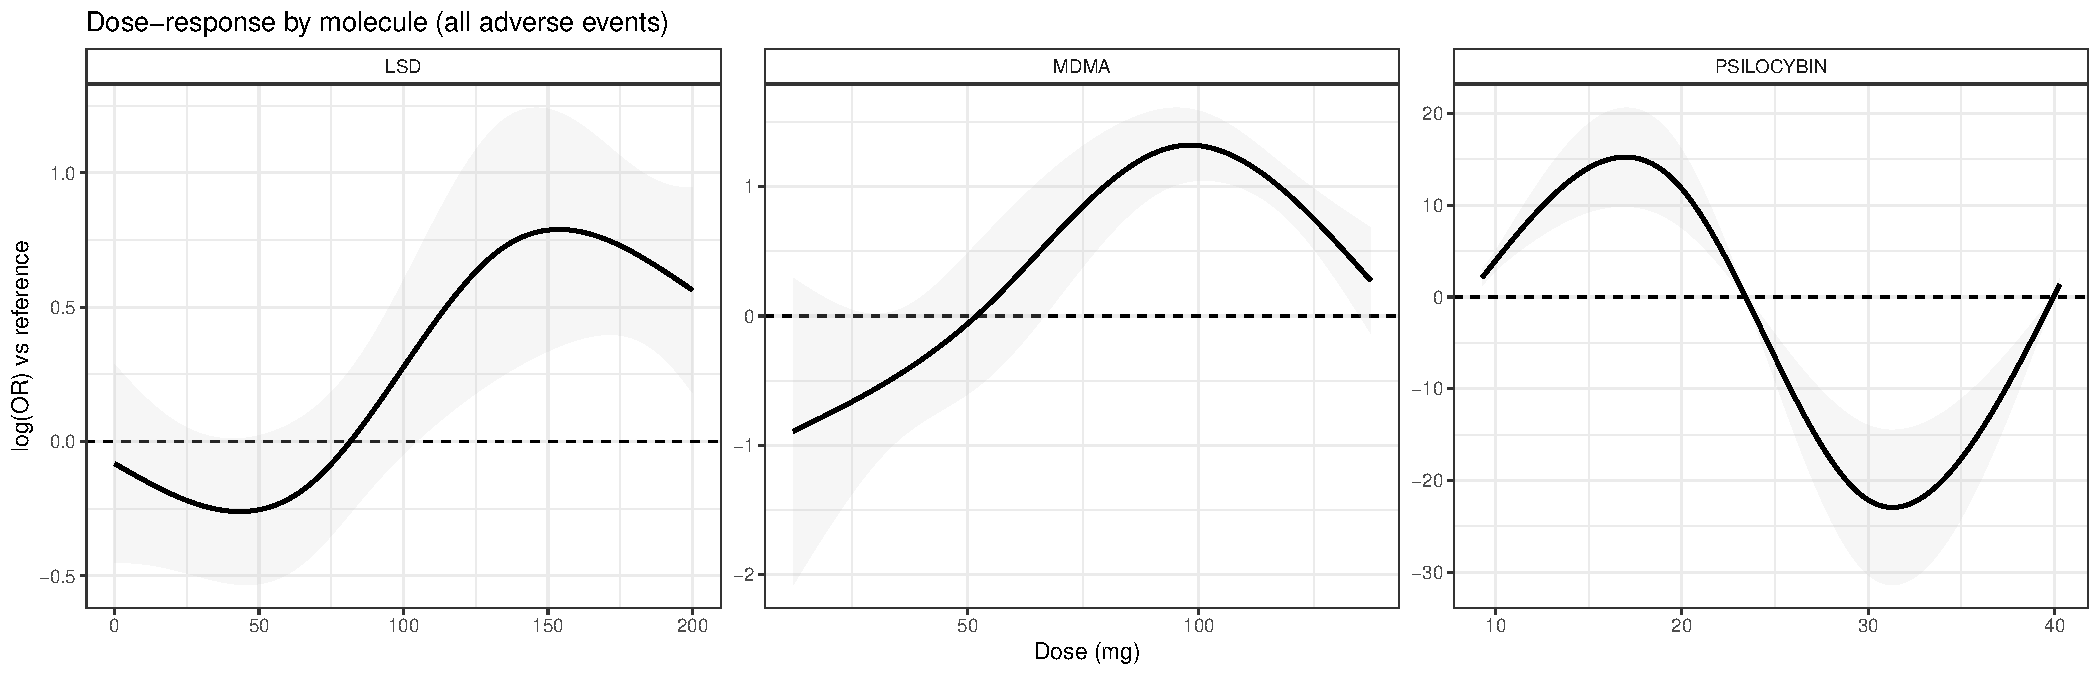
\includegraphics[width=\linewidth]{figures/master_dr_by_molecule-session.pdf}
    \caption{Session-level dose--response curves derived from spline meta-regressions for each molecule.}
    \label{fig:dose-response}
  \end{figure}
}{}

\subsection{Session versus follow-up comparisons}
Comparative analyses of session and follow-up windows highlighted attenuation of effects at later assessments, as visualised in \Cref{fig:session-followup}. Table-based contrasts (\Cref{tab:topline-summary,tab:cmp_ae_molecule}) show that several AE terms with session-level significance did not retain statistical support at follow-up, reflecting limited sample sizes and fewer reported contrasts.

\IfFileExists{figures/dr_session_vs_followup.pdf}{%
  \begin{figure}[ht]
    \centering
    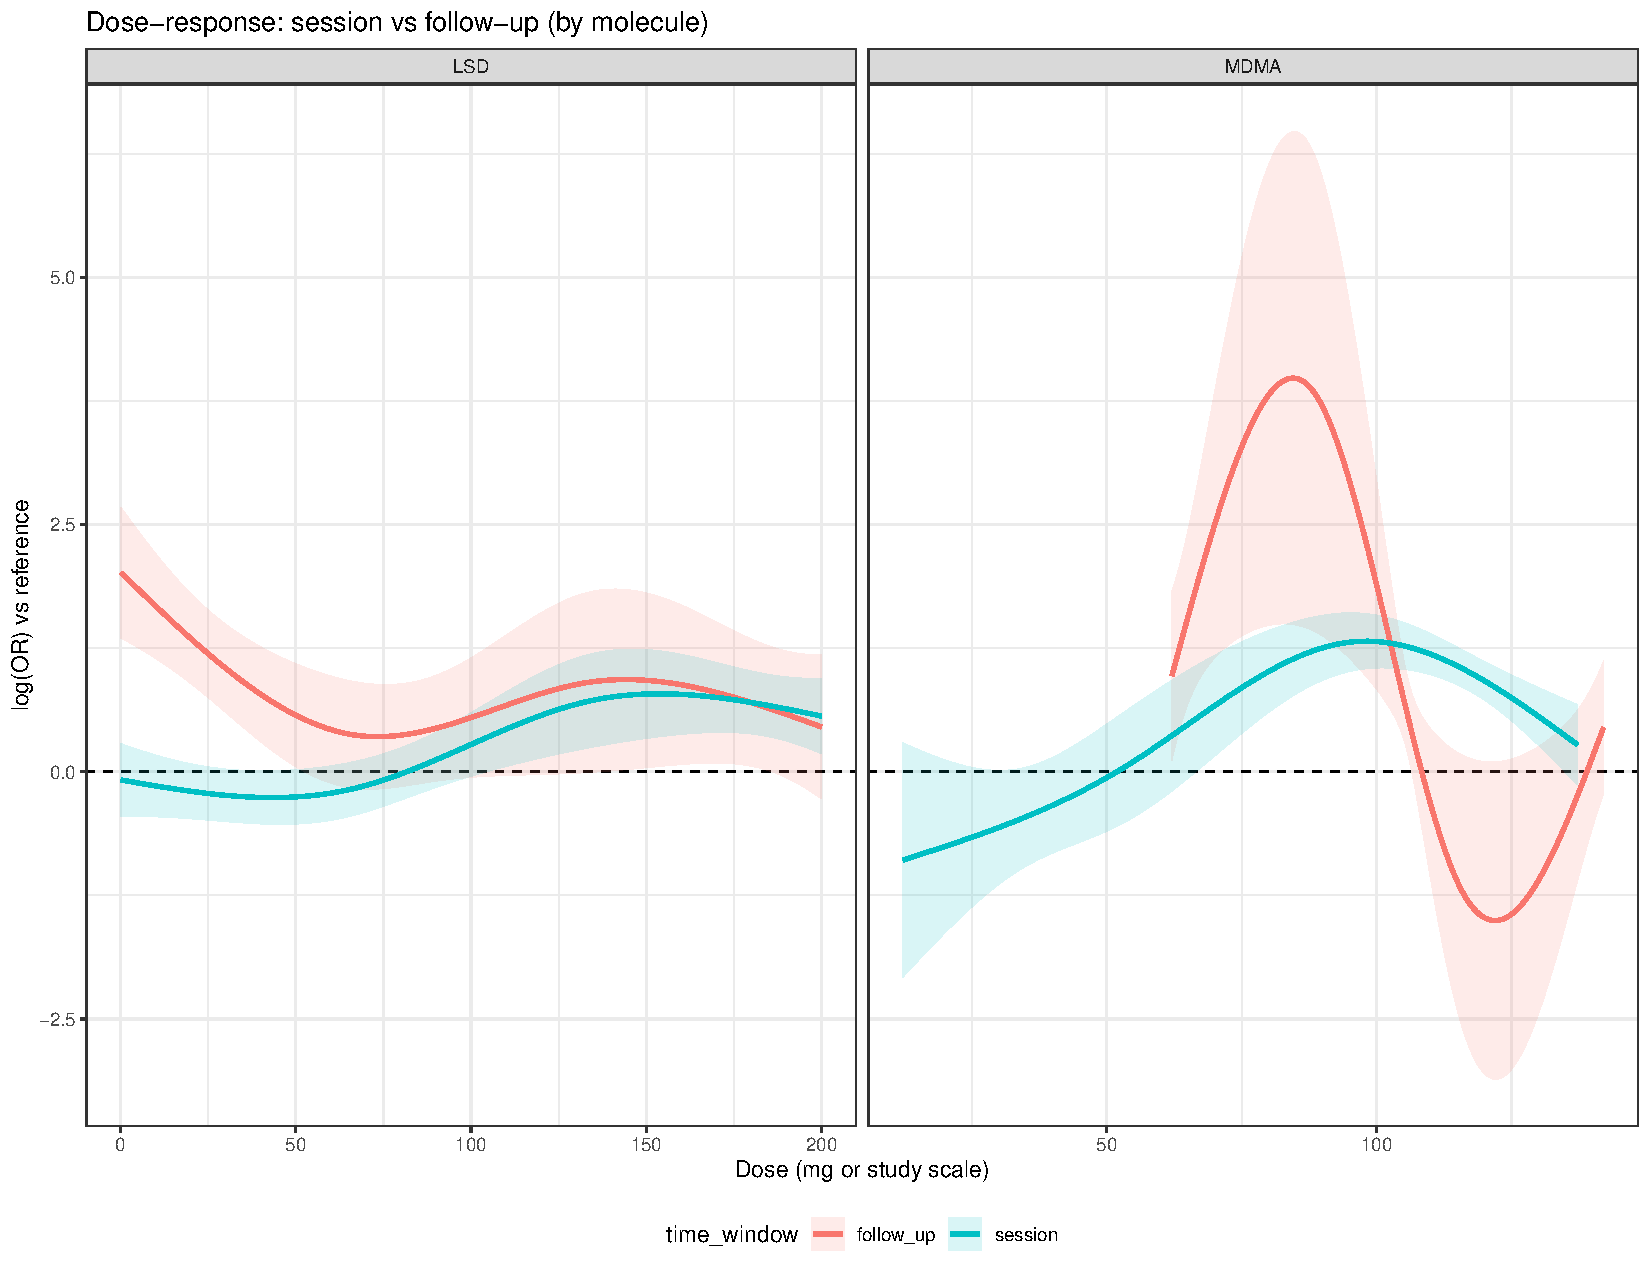
\includegraphics[width=\linewidth]{figures/dr_session_vs_followup.pdf}
    \caption{Comparison of session and follow-up dose--response slopes across molecules.}
    \label{fig:session-followup}
  \end{figure}
}{}

\subsection{Sensitivity and publication-bias assessments}
Leave-one-out diagnostics did not materially change pooled odds ratios for molecules with at least three contributing contrasts, indicating robustness to the exclusion of individual trials. Session-level Egger tests were only feasible for LSD and MDMA because other strata had $k<10$; neither test detected small-study asymmetry at the 0.05 level. Stratified analyses comparing session versus follow-up windows (\Cref{fig:session-followup}) and per-AE contrasts (\Cref{tab:cmp_ae_molecule}) demonstrated that attenuation at follow-up is largely attributable to reduced sample sizes rather than outlying studies.
